$\because$ 2 foci exist for this conic, it must be an ellipse or a hyperbola.
\begin{align}
	\therefore 
	\label{eq:11/11/3/16/F}
	\vec{F}_1 =\myvec{0 \\6}, \vec{F}_2 = \myvec{0 \\-6}, 
	\\
\vec{u} =\frac{\vec{F_1}+\vec{F_2}}{2}=\myvec{0\\0}
\\
\vec{n}\equiv\vec{F_1}-\vec{F_2}\equiv\myvec{0\\1}
	\label{eq:11/11/3/16}
\end{align}
Using 
	\eqref{eq:11/11/3/16}
	in
  \eqref{eq:conic_quad_form_v},
\begin{align}
 \vec{V} = \myvec{1&0\\0&1-e^2}
\end{align}
From \eqref{eq:chord-len-minor}, the length of the minor axis
\begin{align}
 16 = 2\sqrt{\frac{|f|}{|1-e^2|}}
 \\
	\implies
8\sqrt{|1-e^2|}=\sqrt{|f|}
	\label{eq:11/11/3/16/e}
\end{align}
  From \eqref{eq:conic_quad_form_F}, substituting from 
	\eqref{eq:11/11/3/16/F}
	and 
	\eqref{eq:11/11/3/16},
\begin{align}
	\label{eq:11/11/3/16/c1}
\pm ce^2=6
\end{align}
Substituting all known values in
\label{eq:conic_quad_form_nc}, 
\begin{align}
c=\pm\frac{1}{e}\sqrt{\frac{|f|}{|e^2-1|}}
	\label{eq:11/11/3/16/c}
\end{align}
	In \eqref{eq:11/11/3/16/e}-\eqref{eq:11/11/3/16/c}, there are 3 unkowns, $(c, f, e)$.  
Upon solving, we get 
\begin{align}
e=\frac{3}{4}, c=\pm\frac{32}{3}, |f|=28.
\end{align}
Let
\begin{align}
 \vec{x}= \myvec{0 \\ \alpha}
\end{align}
be a vertex of the conic on the minor axis.  Substituting in
    \eqref{eq:conic_quad_form},
\begin{align}
\frac{7\alpha^2}{16}+f=0 \implies f < 0
\\
	\text{or, }
f = -28.
\end{align}
Thus, the desired 
equation of the conic is
\begin{align}
\vec{x}^\top\myvec{1&0\\0&\frac{7}{16}}\vec{x}-28 = 0
\end{align}
See
	\figref{fig:11/11/3/16}.
\begin{figure}[H]
	\centering
	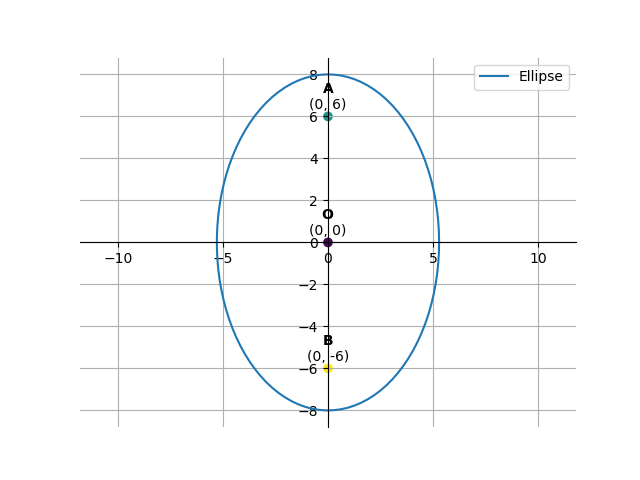
\includegraphics[width=0.75\columnwidth]{chapters/11/11/3/16/figs/fig.png}
	\caption{}
	\label{fig:11/11/3/16}
\end{figure}


